\section{Erdos-Renyi graphs}
The experiments involving Erdos-Renyi graph model is carried out in a similar fashion
as for the grid graph. We consider an Erdo-Renyi graph with 64 nodes, denoted as
$\mathcal{G}^{(64, p)}_{\mathsf{ER}}$, with $p = 0.1$, where $p$ is the probability that
a particular node is connected to any other node.

On what concerns hyperparameter tunning, we fix $\alpha = 1.3\cdot 10^{-2}$ and start with
$\beta = 10^{-1}$ and we exponentially increase it up to $\beta = 1$ for the values of $T$
such that $T / N \leq 1$. For $1 < T / N \leq 30$, we set $\alpha = 0$ and $\beta = 1.5$.
Finally, for $T / N > 30$, we set $\alpha = 0$ and $\beta = 10$.

The hyperparameter tuning for the \textsf{CGL} and \textsf{CGL}$(\mathbf{A})$ algorithms
is done as described for the grid graph model.

Figure~\ref{fig:performance-erdos-renyi} reveals that the algorithms \textsf{SGL}
and \textsf{CGL} obtain a similar performance across the sample size regimes. Unsurprisingly,
the algorithm \textsf{CGL}($\mathbf{A}$) attains nearly perferct F-score for $T / N > 10$,
because, again, it assumes that the connectivity information is fully available, which may be
a non trivial assumption in practice.

\begin{figure}[!htb]
    \centering
    \begin{subfigure}[b]{0.47\textwidth}
      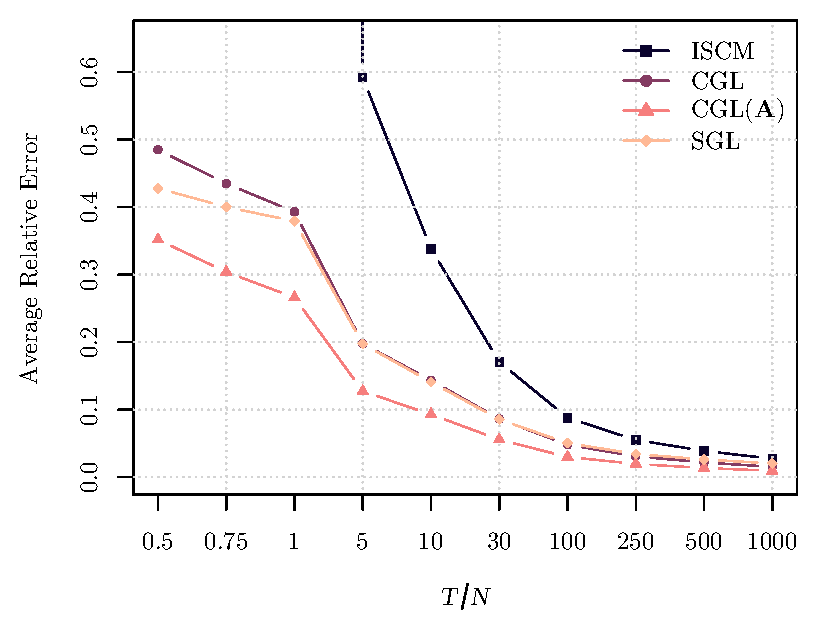
\includegraphics[width=\textwidth]{erdos-renyi/latex/figures/relative_error_erdos_renyi.eps}
    \end{subfigure}
    ~ %add desired spacing between images, e. g. ~, \quad, \qquad, \hfill etc.
      %(or a blank line to force the subfigure onto a new line)
    \begin{subfigure}[b]{0.47\textwidth}
        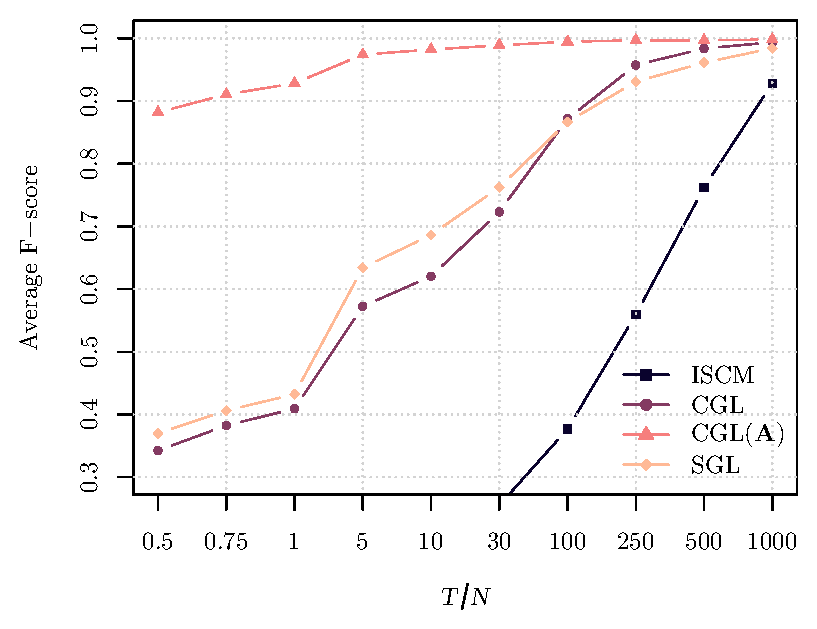
\includegraphics[width=\textwidth]{erdos-renyi/latex/figures/fscore_erdos_renyi.eps}
    \end{subfigure}
    \caption{Average performance results for learning Laplacian matrix of a $\mathcal{G}^{(64, 0.1)}_{\mathsf{ER}}$.}
    \label{fig:performance-erdos-renyi}
\end{figure}

